\section{Resultados y análisis}
\subsection{Simulaciones}
Antes de poner a prueba el proyecto en la vida real, se debe verificar que el programa funcione correctamente con simulaciones. Los archivos referentes a las simulaciones se encuentran en \tt{src/simulide}.
\subsubsection{Pruebas en DC}
Primero se realizó una prueba en DC utilizando como prueba una tensión y corriente de \SI{3.75}{\volt} y \SI{5}{\ampere}. En principio, la potencia consumida es \SI{18.75}{\watt}. La figura \ref{sim-dc} muestra la simulación en DC. Se puede observar que hay una concordancia entre la simulación y el cálculo teórico. Por lo tanto, se concluye que el medidor funciona correctamente en DC.
\begin{figure}[h]
    \centering
    \includegraphics[width=11cm]{Imagenes/sim-dc.png}
    \caption{Simulación del programa en DC.}
    \label{sim-dc}
\end{figure}

\FloatBarrier

\subsubsection{Pruebas en AC}
Ahora, para simular en AC, primero se debe crear un circuito RC para crear una onda desfasada respecto a otra onda \cite{hayt} con el fin de poder comprobar el factor de potencia (figura \ref{oscope}). El desfase de prueba entre ambas ondas es de \SI{45}{\degree}. Además, la ondas amarilla ($N1$) y violenta ($N2$) tienen un valor RMS de 1.76 y 1.24, respectivamente.

\begin{figure}
    \centering
    \includegraphics[width=12cm]{Imagenes/oscope.png}
    \caption{Ondas amarilla y violeta desfasadas \SI{45}{\degree} con un circuito RC para verificar el factor de potencia.}
    \label{oscope}
\end{figure}

Esto quiere decir que para un circuito resistivo (simulado) con la corriente y tensión en fase, la potencia y el factor de potencia son respectivamente \SI{3.125}{\watt} y 1 (teóricos). Ahora, en el caso de un circuito capacitivo e inductivo (simulados) con la corriente y la tensión desfasados \SI{45}{\degree}, la potencia y el factor de potencia son respectivamente \SI{1.54}{\watt} y 0.707 en magnitud (teóricos). Las figuras \ref{sim-res}, \ref{sim-cap} y \ref{sim-ind} ilustran las simulaciones de una carga resistiva, capacitiva e inductiva y sus respectivas mediciones calculados por el software. Nuevamente, se puede observar que el programa calcula correctamente la potencia y el factor de potencia para los tres distintos casos de factor de potencia en AC.

\begin{figure}[h]
    \centering
    \includegraphics[width=11cm]{Imagenes/sim-resistive.png}
    \caption{Simulación del programa en AC con una carga resistiva (corriente y tensión en fase).}
    \label{sim-res}
\end{figure}

\begin{figure}[h]
    \centering
    \includegraphics[width=11cm]{Imagenes/sim-capacitive.png}
    \caption{Simulación del programa en AC con una carga capacitiva (corriente adelantado respecto a la tensión).}
    \label{sim-cap}
\end{figure}

\begin{figure}[h]
    \centering
    \includegraphics[width=11cm]{Imagenes/sim-inductive.png}
    \caption{Simulación del programa en AC con una carga inductiva (corriente atrasado respecto a la tensión).}
    \label{sim-ind}
\end{figure}
\FloatBarrier

\subsection{Pruebas en físico}
\subsubsection{Imprimir las mediciones en el LCD}
Primero se verificó que el programa imprimiera correctamente las mediciones en la pantalla LCD. La figura \ref{imprimir} ilustra que el programa es capaz de mostrar los valores en pantalla sin problema.
\begin{figure}[h]
    \centering
    \includegraphics[width=10cm]{Imagenes/Medicion_Pantalla.jpg}
    \caption{Mediciones impresas en la pantalla LCD.}
    \label{imprimir}
\end{figure}
\FloatBarrier

\subsubsection{Medición de tensión en AC}
Ahora, se procedió a medir la tensión en AC. Con un generador de señales se creó una tensión con \SI{1.03}{\volt}. La figura \ref{voltage-low-ac} muestra el resultado medido por el Arduino (\SI{1.07}{\volt}) y esto fue un buen resultado.
\begin{figure}[h]
    \centering
    \includegraphics[width=12cm]{Imagenes/Tension_AC.jpg}
    \caption{Prueba en la vida real de la tensión en AC.}
    \label{voltage-low-ac}
\end{figure}
\FloatBarrier

\subsubsection{Medición de tensión en DC}
Luego, se probó en DC con una tensión de \SI{3.3}{\volt}. El valor medido en DC por el Arduino se muestra en la figura \ref{voltage-low-dc}. Se observa que el programa calcula correctamente la tensión en DC. Además, se puede observar que con una corriente de \SI{5}{\ampere}, el programa calcula la potencia correctamente.
\begin{figure}[h]
    \centering
    \includegraphics[width=12cm]{Imagenes/Tension_DC.jpg}
    \caption{Prueba en la vida real de la tensión en DC.}
    \label{voltage-low-dc}
\end{figure}
\FloatBarrier
\subsubsection{Medición de corriente}
Para la medición de corriente se tuvo muchos inconvenientes ya que el sensor de corriente conseguido no era capaz de detectar corriente en el orden de los milliamperios (este rango de corriente es típico en circuitos y aplicaciones de baja potencia). Ante este problema, se consultó alternativas al sensor de corrientes al profesor Francisco Escobar, docente de sistemas de potencia de la escuela de Ingeniería eléctrica. Él sugirió utilizar un transformador de corriente (figura \ref{flexifomer}) como una alternativa al sensor de corriente. El funcionamiento y teoría del transformador de corriente se puede consultar en la sección de anexos.

\begin{figure}
    \centering
    \includegraphics[width=10cm]{Imagenes/flexiformer.jpeg}
    \caption{Transformador de corriente.}
    \label{flexifomer}
\end{figure}

\begin{figure}
    \centering
    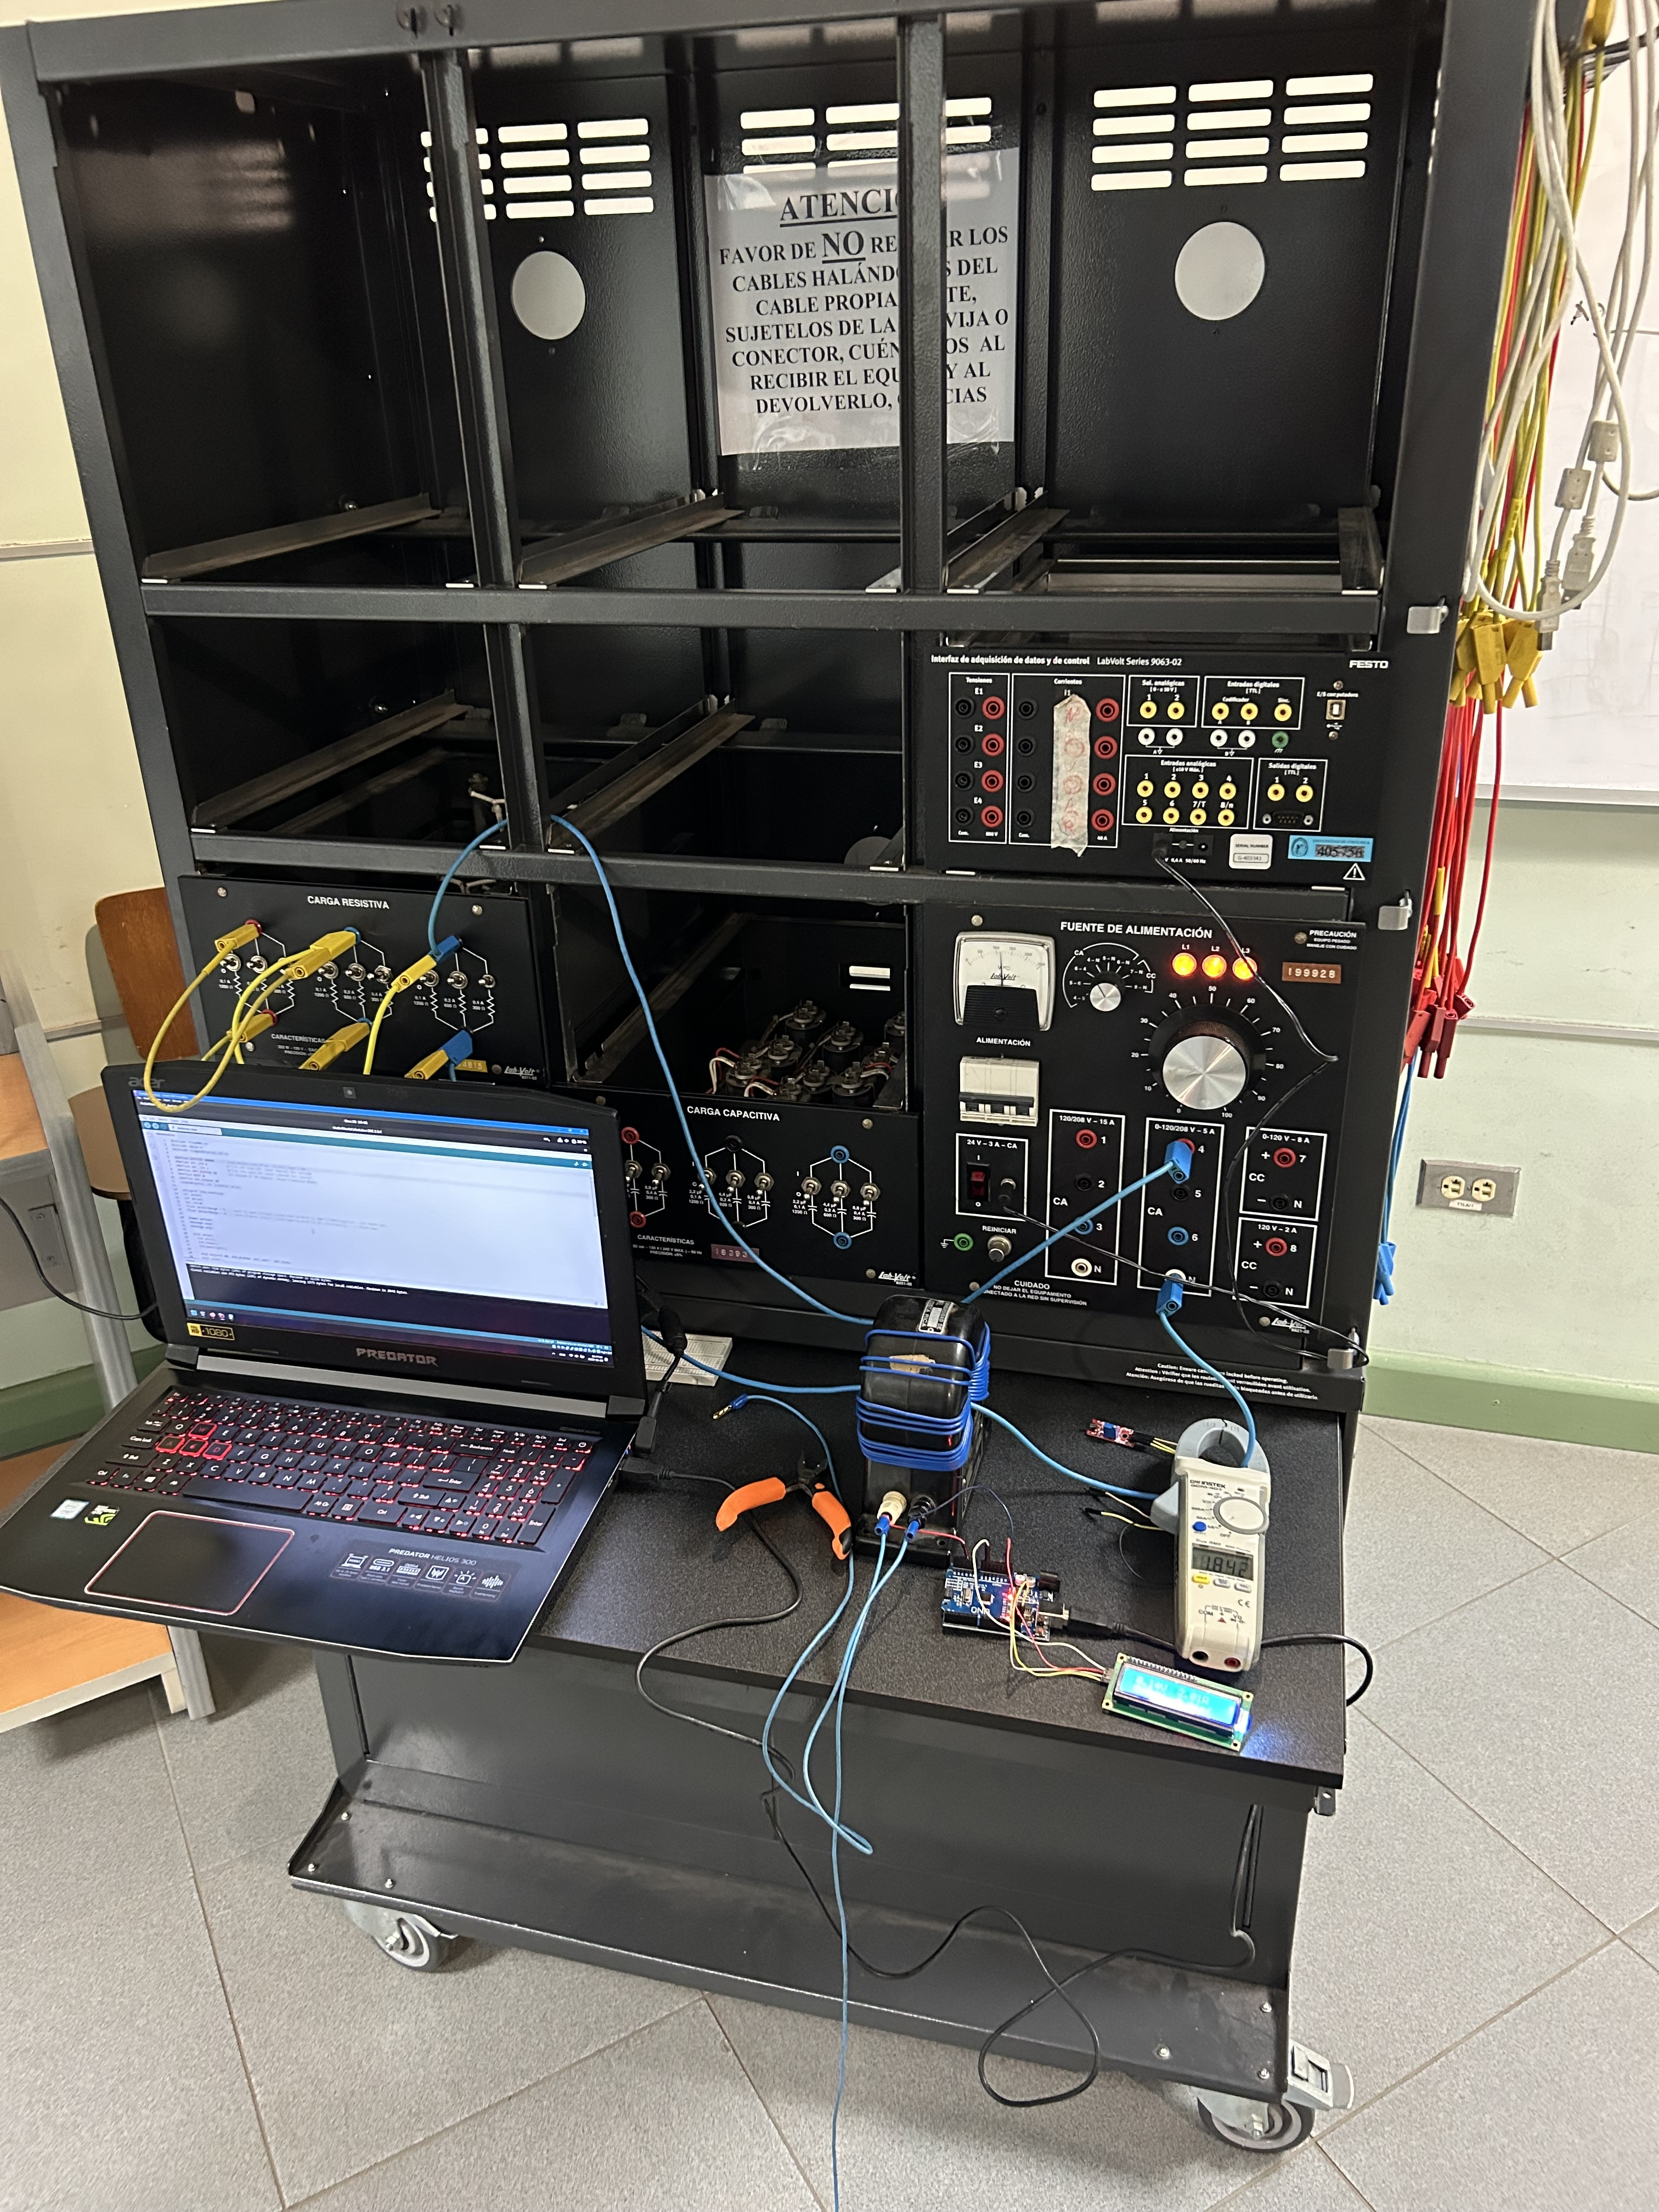
\includegraphics[width=12cm]{Imagenes/current.jpg}
    \caption{Setup en el laboratorio de máquinas eléctricas para probar la medición de corriente con el transformador de corriente.}
    \label{current-test}
\end{figure}

Por lo tanto, se decidió seguir la recomendación del profesor y probar la sugerencia. En la figura \ref{current-test} se puede observar un setup en el laboratorio de máquinas eléctricas para llevar a cabo la sugerencia. Finalmente, en la figura \ref{current-res} se observa que se obtuvo buenas mediciones de corriente. Al obtenerse buenas mediciones de corriente, se decidió cambiar el alcance del proyecto, en vez de medir aplicaciones de baja potencia en AC y DC, medir aplicaciones de alta potencia solamente en AC. Esto se debe a que el transformador de corriente funciona generalmente para aplicaciones de alta potencia y por la ley de inducción de Faraday solo sirve en AC \cite{hayt}. 

\begin{figure}
    \centering
    \begin{subfigure}{0.45\textwidth}
        \includegraphics[width=\textwidth]{Imagenes/corriente1.jpeg}
    \end{subfigure}
    \begin{subfigure}{0.45\textwidth}
        \includegraphics[width=\textwidth]{Imagenes/corriente2.jpeg}
    \end{subfigure}
    \caption{Medición de corriente de un circuito de alta potencia con el transformador de corriente.}
    \label{current-res}
\end{figure}

\subsubsection{Medición de potencia (alta potencia)}
Como se comentó anteriormente, el proyecto cambió su enfoque para medir aplicaciones de alta potencia. Esto implica que el circuito resistivo diseñado (figura \ref{hardware}) ya no funcionará, puesto que se necesita aislar eléctricamente el circuito de alta potencia del Arduino para evitar que se dañe. En su lugar, se utilizó un transformador reductor para poder medir la tensión de alta potencia \cite{hayt}.

\begin{figure}[h]
    \centering
    \includegraphics[width=\textwidth]{Imagenes/Circuito_completo.jpg}
    \caption{Setup en el laboratorio de máquinas eléctricas para medir la potencia y factor de potencia.}
    \label{setup-watt}
\end{figure}
\FloatBarrier

Ahora, la figura \ref{setup-watt} ilustra el setup utilizado para medir la potencia y factor de potencia de circuitos de alta potencia en AC. En este setup se probó los tres casos posibles de un circuito en AC, un circuito resistivo, un circuito capacitivo y un circuito inductivo \cite{hayt}.

\begin{figure}[h]
    \centering
    \begin{subfigure}{0.45\textwidth}
        \includegraphics[width=\textwidth]{Imagenes/resistive.jpg}
        \caption{Valor teórico.}
    \end{subfigure}
    \begin{subfigure}{0.45\textwidth}
        \includegraphics[width=\textwidth]{Imagenes/resistive_2.jpg} 
        \caption{Valor medido.}
    \end{subfigure}
    \caption{Valores teórico (\SI{118.11}{\volt} y \SI{2.07}{\ampere}) y medido (\SI{126.57}{\volt}
    y \SI{1.59}{\ampere}) de un circuito resistivo.}
    \label{res--}
\end{figure}

\FloatBarrier

Como se puede observar en la figuras \ref{res--}, \ref{cap--} y \ref{ind--}, el Arduino logra medir la tensión y corriente, así como calcular la potencia y factor de potencia en cada caso. Sin embargo, se puede observar que las mediciones de tensión y corriente contiene cierto error de medición, siendo la medición de corriente la más grave. Más grave aún es la medición del factor de potencia, donde en principio debe ser 1 para el circuito resistivo y 0.707 para los circuitos capacitivo e inductivo. Sin embargo, el factor de potencia reportado por el Arduino no son los esperados al compararse con los valores teóricos.

\begin{figure}[h]
    \centering
    \begin{subfigure}{0.45\textwidth}
        \includegraphics[width=\textwidth]{Imagenes/capacitive.jpg}
        \caption{Valor teórico.}
    \end{subfigure}
    \begin{subfigure}{0.45\textwidth}
        \includegraphics[width=\textwidth]{Imagenes/capacitive_2.jpg} 
        \caption{Valor medido.}
    \end{subfigure}
    \caption{Valores teórico (\SI{118.07}{\volt} y \SI{2.91}{\ampere}) y medido (\SI{122.17}{\volt}
    y \SI{2.19}{\ampere}) de un circuito capacitivo.}
    \label{cap--}
\end{figure}


\begin{figure}[h]
    \centering
    \begin{subfigure}{0.45\textwidth}
        \includegraphics[width=\textwidth]{Imagenes/inductive.jpg}
        \caption{Valor teórico.}
    \end{subfigure}
    \begin{subfigure}{0.45\textwidth}
        \includegraphics[width=\textwidth]{Imagenes/inductive_2.jpg} 
        \caption{Valor medido.}
    \end{subfigure}
    \caption{Valores teórico (\SI{117.81}{\volt} y \SI{3.06}{\ampere}) y medido (\SI{125.81}{\volt}
    y \SI{2.45}{\ampere}) de un circuito inductivo.}
    \label{ind--}
\end{figure}

Una posible causa de este error puede ser una interferencia eléctrica donde el transformador afecte al transformador de corriente o viceversa, y a su vez afecte las mediciones de tensión y corriente. Esto se debe a que al medir la tensión y corriente por separados, no hubo este tipo de problema. Además, se descarta que el problema sea a nivel de software, ya que se verificó mediante simulaciones que el software sí funciona correctamente. Por último, por falta de tiempo no se pudo resolver todos los problemas que surgieron durante el desarrollo de este proyecto, pero sí se pudo cumplir los objetivos propuestos del proyecto.
\FloatBarrier


































